% Options for packages loaded elsewhere
\PassOptionsToPackage{unicode}{hyperref}
\PassOptionsToPackage{hyphens}{url}
%
\documentclass[
  landscape]{article}
\usepackage{amsmath,amssymb}
\usepackage{lmodern}
\usepackage{ifxetex,ifluatex}
\ifnum 0\ifxetex 1\fi\ifluatex 1\fi=0 % if pdftex
  \usepackage[T1]{fontenc}
  \usepackage[utf8]{inputenc}
  \usepackage{textcomp} % provide euro and other symbols
\else % if luatex or xetex
  \usepackage{unicode-math}
  \defaultfontfeatures{Scale=MatchLowercase}
  \defaultfontfeatures[\rmfamily]{Ligatures=TeX,Scale=1}
\fi
% Use upquote if available, for straight quotes in verbatim environments
\IfFileExists{upquote.sty}{\usepackage{upquote}}{}
\IfFileExists{microtype.sty}{% use microtype if available
  \usepackage[]{microtype}
  \UseMicrotypeSet[protrusion]{basicmath} % disable protrusion for tt fonts
}{}
\makeatletter
\@ifundefined{KOMAClassName}{% if non-KOMA class
  \IfFileExists{parskip.sty}{%
    \usepackage{parskip}
  }{% else
    \setlength{\parindent}{0pt}
    \setlength{\parskip}{6pt plus 2pt minus 1pt}}
}{% if KOMA class
  \KOMAoptions{parskip=half}}
\makeatother
\usepackage{xcolor}
\IfFileExists{xurl.sty}{\usepackage{xurl}}{} % add URL line breaks if available
\IfFileExists{bookmark.sty}{\usepackage{bookmark}}{\usepackage{hyperref}}
\hypersetup{
  hidelinks,
  pdfcreator={LaTeX via pandoc}}
\urlstyle{same} % disable monospaced font for URLs
\usepackage[margin=1in]{geometry}
\usepackage{color}
\usepackage{fancyvrb}
\newcommand{\VerbBar}{|}
\newcommand{\VERB}{\Verb[commandchars=\\\{\}]}
\DefineVerbatimEnvironment{Highlighting}{Verbatim}{commandchars=\\\{\}}
% Add ',fontsize=\small' for more characters per line
\usepackage{framed}
\definecolor{shadecolor}{RGB}{248,248,248}
\newenvironment{Shaded}{\begin{snugshade}}{\end{snugshade}}
\newcommand{\AlertTok}[1]{\textcolor[rgb]{0.94,0.16,0.16}{#1}}
\newcommand{\AnnotationTok}[1]{\textcolor[rgb]{0.56,0.35,0.01}{\textbf{\textit{#1}}}}
\newcommand{\AttributeTok}[1]{\textcolor[rgb]{0.77,0.63,0.00}{#1}}
\newcommand{\BaseNTok}[1]{\textcolor[rgb]{0.00,0.00,0.81}{#1}}
\newcommand{\BuiltInTok}[1]{#1}
\newcommand{\CharTok}[1]{\textcolor[rgb]{0.31,0.60,0.02}{#1}}
\newcommand{\CommentTok}[1]{\textcolor[rgb]{0.56,0.35,0.01}{\textit{#1}}}
\newcommand{\CommentVarTok}[1]{\textcolor[rgb]{0.56,0.35,0.01}{\textbf{\textit{#1}}}}
\newcommand{\ConstantTok}[1]{\textcolor[rgb]{0.00,0.00,0.00}{#1}}
\newcommand{\ControlFlowTok}[1]{\textcolor[rgb]{0.13,0.29,0.53}{\textbf{#1}}}
\newcommand{\DataTypeTok}[1]{\textcolor[rgb]{0.13,0.29,0.53}{#1}}
\newcommand{\DecValTok}[1]{\textcolor[rgb]{0.00,0.00,0.81}{#1}}
\newcommand{\DocumentationTok}[1]{\textcolor[rgb]{0.56,0.35,0.01}{\textbf{\textit{#1}}}}
\newcommand{\ErrorTok}[1]{\textcolor[rgb]{0.64,0.00,0.00}{\textbf{#1}}}
\newcommand{\ExtensionTok}[1]{#1}
\newcommand{\FloatTok}[1]{\textcolor[rgb]{0.00,0.00,0.81}{#1}}
\newcommand{\FunctionTok}[1]{\textcolor[rgb]{0.00,0.00,0.00}{#1}}
\newcommand{\ImportTok}[1]{#1}
\newcommand{\InformationTok}[1]{\textcolor[rgb]{0.56,0.35,0.01}{\textbf{\textit{#1}}}}
\newcommand{\KeywordTok}[1]{\textcolor[rgb]{0.13,0.29,0.53}{\textbf{#1}}}
\newcommand{\NormalTok}[1]{#1}
\newcommand{\OperatorTok}[1]{\textcolor[rgb]{0.81,0.36,0.00}{\textbf{#1}}}
\newcommand{\OtherTok}[1]{\textcolor[rgb]{0.56,0.35,0.01}{#1}}
\newcommand{\PreprocessorTok}[1]{\textcolor[rgb]{0.56,0.35,0.01}{\textit{#1}}}
\newcommand{\RegionMarkerTok}[1]{#1}
\newcommand{\SpecialCharTok}[1]{\textcolor[rgb]{0.00,0.00,0.00}{#1}}
\newcommand{\SpecialStringTok}[1]{\textcolor[rgb]{0.31,0.60,0.02}{#1}}
\newcommand{\StringTok}[1]{\textcolor[rgb]{0.31,0.60,0.02}{#1}}
\newcommand{\VariableTok}[1]{\textcolor[rgb]{0.00,0.00,0.00}{#1}}
\newcommand{\VerbatimStringTok}[1]{\textcolor[rgb]{0.31,0.60,0.02}{#1}}
\newcommand{\WarningTok}[1]{\textcolor[rgb]{0.56,0.35,0.01}{\textbf{\textit{#1}}}}
\usepackage{longtable,booktabs,array}
\usepackage{calc} % for calculating minipage widths
% Correct order of tables after \paragraph or \subparagraph
\usepackage{etoolbox}
\makeatletter
\patchcmd\longtable{\par}{\if@noskipsec\mbox{}\fi\par}{}{}
\makeatother
% Allow footnotes in longtable head/foot
\IfFileExists{footnotehyper.sty}{\usepackage{footnotehyper}}{\usepackage{footnote}}
\makesavenoteenv{longtable}
\usepackage{graphicx}
\makeatletter
\def\maxwidth{\ifdim\Gin@nat@width>\linewidth\linewidth\else\Gin@nat@width\fi}
\def\maxheight{\ifdim\Gin@nat@height>\textheight\textheight\else\Gin@nat@height\fi}
\makeatother
% Scale images if necessary, so that they will not overflow the page
% margins by default, and it is still possible to overwrite the defaults
% using explicit options in \includegraphics[width, height, ...]{}
\setkeys{Gin}{width=\maxwidth,height=\maxheight,keepaspectratio}
% Set default figure placement to htbp
\makeatletter
\def\fps@figure{htbp}
\makeatother
\setlength{\emergencystretch}{3em} % prevent overfull lines
\providecommand{\tightlist}{%
  \setlength{\itemsep}{0pt}\setlength{\parskip}{0pt}}
\setcounter{secnumdepth}{-\maxdimen} % remove section numbering
\ifluatex
  \usepackage{selnolig}  % disable illegal ligatures
\fi

\title{Logistics data analysis using R programming\\
{[}202102-LSB5019-001{]}\\
~\\
Assignment 4}
\author{QIA WANG\\
(91219618)}
\date{2021-11-04}

\begin{document}
\maketitle

\#1) Load the price index .csv file attached via this
assignment\#\#\#\#\#\#\#\#\#\#\#\#\#\#\#\#\#\#\#\#\#\#\#\#\#

\begin{Shaded}
\begin{Highlighting}[]
\NormalTok{destfile}\OtherTok{\textless{}{-}} \StringTok{"D:}\SpecialCharTok{\textbackslash{}\textbackslash{}}\StringTok{One}\SpecialCharTok{\textbackslash{}\textbackslash{}}\StringTok{OneDrive}\SpecialCharTok{\textbackslash{}\textbackslash{}}\StringTok{My research}\SpecialCharTok{\textbackslash{}\textbackslash{}}\StringTok{5th semester}\SpecialCharTok{\textbackslash{}\textbackslash{}}\StringTok{R}\SpecialCharTok{\textbackslash{}\textbackslash{}}\StringTok{Assignment 4}\SpecialCharTok{\textbackslash{}\textbackslash{}}\StringTok{food{-}price{-}index{-}September{-}2021{-}index{-}numbers{-}csv{-}tables.csv"}
\NormalTok{pricedata}\OtherTok{\textless{}{-}} \FunctionTok{read.csv}\NormalTok{(destfile) }\CommentTok{\#load the file}
\end{Highlighting}
\end{Shaded}

\#2) Use 4 methods that you learned in the last two sessions to
manipulate the dataset\#\#\#\#

\begin{Shaded}
\begin{Highlighting}[]
\CommentTok{\#2.1: read the data file and overview its content (library(data.table))}
\FunctionTok{head}\NormalTok{(pricedata,}\AttributeTok{n=}\DecValTok{3}\NormalTok{) }\CommentTok{\# check the first 3 rows}
\end{Highlighting}
\end{Shaded}

\begin{longtable}[]{@{}
  >{\raggedright\arraybackslash}p{(\columnwidth - 14\tabcolsep) * \real{0.10}}
  >{\raggedleft\arraybackslash}p{(\columnwidth - 14\tabcolsep) * \real{0.05}}
  >{\raggedleft\arraybackslash}p{(\columnwidth - 14\tabcolsep) * \real{0.07}}
  >{\raggedright\arraybackslash}p{(\columnwidth - 14\tabcolsep) * \real{0.04}}
  >{\raggedright\arraybackslash}p{(\columnwidth - 14\tabcolsep) * \real{0.05}}
  >{\raggedright\arraybackslash}p{(\columnwidth - 14\tabcolsep) * \real{0.17}}
  >{\raggedright\arraybackslash}p{(\columnwidth - 14\tabcolsep) * \real{0.44}}
  >{\raggedright\arraybackslash}p{(\columnwidth - 14\tabcolsep) * \real{0.09}}@{}}
\toprule
Series\_reference & Period & Data\_value & STATUS & UNITS & Subject &
Group & Series\_title\_1 \\
\midrule
\endhead
CPIM.SAP0100 & 2006.06 & 3.11 & FINAL & Dollars & Consumers Price Index
- CPI & Food Price Index Selected Monthly Weighted Average Prices for
New Zealand & Oranges, 1kg \\
CPIM.SAP0100 & 2006.07 & 2.78 & FINAL & Dollars & Consumers Price Index
- CPI & Food Price Index Selected Monthly Weighted Average Prices for
New Zealand & Oranges, 1kg \\
CPIM.SAP0100 & 2006.08 & 2.43 & FINAL & Dollars & Consumers Price Index
- CPI & Food Price Index Selected Monthly Weighted Average Prices for
New Zealand & Oranges, 1kg \\
\bottomrule
\end{longtable}

\begin{Shaded}
\begin{Highlighting}[]
\FunctionTok{tail}\NormalTok{(pricedata,}\AttributeTok{n=}\DecValTok{10}\NormalTok{)}\CommentTok{\# check the last 10 rows}
\end{Highlighting}
\end{Shaded}

\begin{longtable}[]{@{}
  >{\raggedright\arraybackslash}p{(\columnwidth - 16\tabcolsep) * \real{0.03}}
  >{\raggedright\arraybackslash}p{(\columnwidth - 16\tabcolsep) * \real{0.09}}
  >{\raggedleft\arraybackslash}p{(\columnwidth - 16\tabcolsep) * \real{0.04}}
  >{\raggedleft\arraybackslash}p{(\columnwidth - 16\tabcolsep) * \real{0.06}}
  >{\raggedright\arraybackslash}p{(\columnwidth - 16\tabcolsep) * \real{0.04}}
  >{\raggedright\arraybackslash}p{(\columnwidth - 16\tabcolsep) * \real{0.04}}
  >{\raggedright\arraybackslash}p{(\columnwidth - 16\tabcolsep) * \real{0.15}}
  >{\raggedright\arraybackslash}p{(\columnwidth - 16\tabcolsep) * \real{0.40}}
  >{\raggedright\arraybackslash}p{(\columnwidth - 16\tabcolsep) * \real{0.14}}@{}}
\toprule
& Series\_reference & Period & Data\_value & STATUS & UNITS & Subject &
Group & Series\_title\_1 \\
\midrule
\endhead
25954 & CPIM.SAP0269 & 2020.12 & 3.08 & FINAL & Dollars & Consumers
Price Index - CPI & Food Price Index Selected Monthly Weighted Average
Prices for New Zealand & Chewing gum, packet, each \\
25955 & CPIM.SAP0269 & 2021.01 & 3.10 & FINAL & Dollars & Consumers
Price Index - CPI & Food Price Index Selected Monthly Weighted Average
Prices for New Zealand & Chewing gum, packet, each \\
25956 & CPIM.SAP0269 & 2021.02 & 3.09 & FINAL & Dollars & Consumers
Price Index - CPI & Food Price Index Selected Monthly Weighted Average
Prices for New Zealand & Chewing gum, packet, each \\
25957 & CPIM.SAP0269 & 2021.03 & 3.10 & FINAL & Dollars & Consumers
Price Index - CPI & Food Price Index Selected Monthly Weighted Average
Prices for New Zealand & Chewing gum, packet, each \\
25958 & CPIM.SAP0269 & 2021.04 & 3.08 & FINAL & Dollars & Consumers
Price Index - CPI & Food Price Index Selected Monthly Weighted Average
Prices for New Zealand & Chewing gum, packet, each \\
25959 & CPIM.SAP0269 & 2021.05 & 3.12 & FINAL & Dollars & Consumers
Price Index - CPI & Food Price Index Selected Monthly Weighted Average
Prices for New Zealand & Chewing gum, packet, each \\
25960 & CPIM.SAP0269 & 2021.06 & 3.16 & FINAL & Dollars & Consumers
Price Index - CPI & Food Price Index Selected Monthly Weighted Average
Prices for New Zealand & Chewing gum, packet, each \\
25961 & CPIM.SAP0269 & 2021.07 & 3.10 & FINAL & Dollars & Consumers
Price Index - CPI & Food Price Index Selected Monthly Weighted Average
Prices for New Zealand & Chewing gum, packet, each \\
25962 & CPIM.SAP0269 & 2021.08 & 3.13 & FINAL & Dollars & Consumers
Price Index - CPI & Food Price Index Selected Monthly Weighted Average
Prices for New Zealand & Chewing gum, packet, each \\
25963 & CPIM.SAP0269 & 2021.09 & 3.16 & FINAL & Dollars & Consumers
Price Index - CPI & Food Price Index Selected Monthly Weighted Average
Prices for New Zealand & Chewing gum, packet, each \\
\bottomrule
\end{longtable}

\begin{Shaded}
\begin{Highlighting}[]
\FunctionTok{summary}\NormalTok{(pricedata) }\CommentTok{\# summary of the object}
\end{Highlighting}
\end{Shaded}

\begin{verbatim}
##  Series_reference       Period       Data_value        STATUS         
##  Length:25963       Min.   :2006   Min.   : 0.900   Length:25963      
##  Class :character   1st Qu.:2010   1st Qu.: 2.640   Class :character  
##  Mode  :character   Median :2014   Median : 3.660   Mode  :character  
##                     Mean   :2014   Mean   : 5.432                     
##                     3rd Qu.:2018   3rd Qu.: 6.160                     
##                     Max.   :2021   Max.   :37.960                     
##                                    NA's   :82                         
##     UNITS             Subject             Group           Series_title_1    
##  Length:25963       Length:25963       Length:25963       Length:25963      
##  Class :character   Class :character   Class :character   Class :character  
##  Mode  :character   Mode  :character   Mode  :character   Mode  :character  
##                                                                             
##                                                                             
##                                                                             
## 
\end{verbatim}

\begin{Shaded}
\begin{Highlighting}[]
\FunctionTok{dim}\NormalTok{(pricedata) }\CommentTok{\# check the dimension}
\end{Highlighting}
\end{Shaded}

\begin{verbatim}
## [1] 25963     8
\end{verbatim}

\begin{Shaded}
\begin{Highlighting}[]
\FunctionTok{names}\NormalTok{(pricedata) }\CommentTok{\# check the object names}
\end{Highlighting}
\end{Shaded}

\begin{verbatim}
## [1] "Series_reference" "Period"           "Data_value"       "STATUS"          
## [5] "UNITS"            "Subject"          "Group"            "Series_title_1"
\end{verbatim}

\begin{Shaded}
\begin{Highlighting}[]
\FunctionTok{str}\NormalTok{(pricedata)}\CommentTok{\# the structure}
\end{Highlighting}
\end{Shaded}

\begin{verbatim}
## 'data.frame':    25963 obs. of  8 variables:
##  $ Series_reference: chr  "CPIM.SAP0100" "CPIM.SAP0100" "CPIM.SAP0100" "CPIM.SAP0100" ...
##  $ Period          : num  2006 2006 2006 2006 2006 ...
##  $ Data_value      : num  3.11 2.78 2.43 2.42 3.04 3.24 3.27 3.18 3.74 4.21 ...
##  $ STATUS          : chr  "FINAL" "FINAL" "FINAL" "FINAL" ...
##  $ UNITS           : chr  "Dollars" "Dollars" "Dollars" "Dollars" ...
##  $ Subject         : chr  "Consumers Price Index - CPI" "Consumers Price Index - CPI" "Consumers Price Index - CPI" "Consumers Price Index - CPI" ...
##  $ Group           : chr  "Food Price Index Selected Monthly Weighted Average Prices for New Zealand" "Food Price Index Selected Monthly Weighted Average Prices for New Zealand" "Food Price Index Selected Monthly Weighted Average Prices for New Zealand" "Food Price Index Selected Monthly Weighted Average Prices for New Zealand" ...
##  $ Series_title_1  : chr  "Oranges, 1kg" "Oranges, 1kg" "Oranges, 1kg" "Oranges, 1kg" ...
\end{verbatim}

\begin{Shaded}
\begin{Highlighting}[]
\CommentTok{\#attributes(pricedata)\# object\textquotesingle{}s attributes}
\FunctionTok{hist}\NormalTok{(pricedata}\SpecialCharTok{$}\NormalTok{Data\_value)}\CommentTok{\# Use a histogram to display data distribution}
\end{Highlighting}
\end{Shaded}

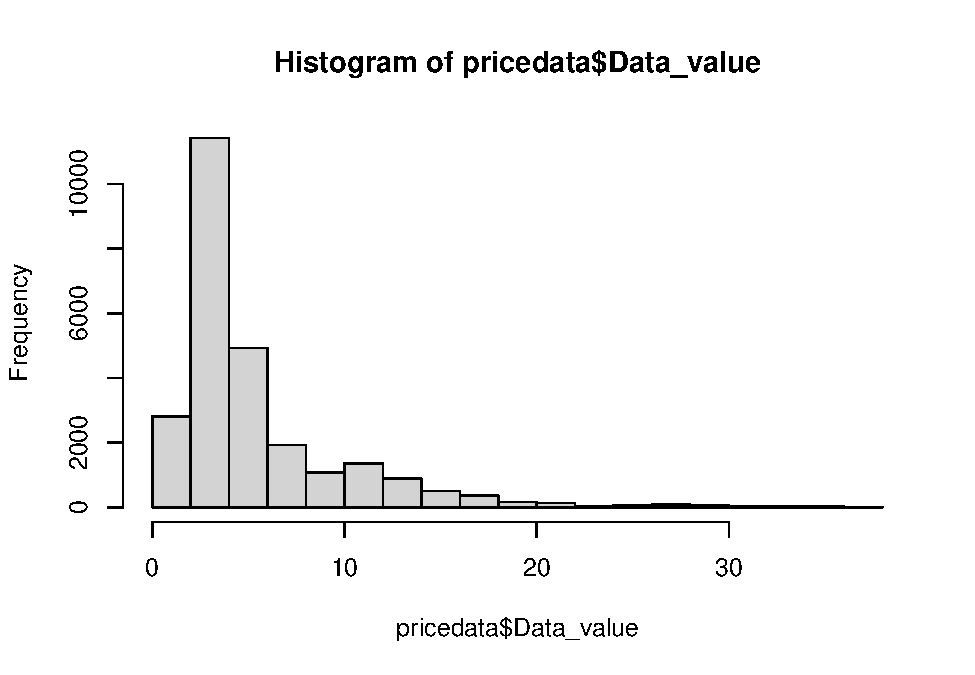
\includegraphics{PDF_files/figure-latex/unnamed-chunk-2-1.pdf}

\begin{Shaded}
\begin{Highlighting}[]
\FunctionTok{table}\NormalTok{(pricedata}\SpecialCharTok{$}\NormalTok{Data\_value)[}\DecValTok{1}\SpecialCharTok{:}\DecValTok{5}\NormalTok{] }\CommentTok{\# Frequency of occurrence of the first 5 values}
\end{Highlighting}
\end{Shaded}

\begin{verbatim}
## 
##  0.9 0.91 0.93 0.94 0.95 
##    1    1    1    1    4
\end{verbatim}

\begin{Shaded}
\begin{Highlighting}[]
\FunctionTok{is.factor}\NormalTok{(pricedata}\SpecialCharTok{$}\NormalTok{Series\_title\_1) }\CommentTok{\# Determine whether it is factor data}
\end{Highlighting}
\end{Shaded}

\begin{verbatim}
## [1] FALSE
\end{verbatim}

\begin{Shaded}
\begin{Highlighting}[]
\CommentTok{\#as.factor(pricedata$Series\_title\_1) \# Convert to factor data}

\CommentTok{\#2.2: Remove the missing data}
\FunctionTok{colSums}\NormalTok{(}\FunctionTok{is.na}\NormalTok{(pricedata))}
\end{Highlighting}
\end{Shaded}

\begin{verbatim}
## Series_reference           Period       Data_value           STATUS 
##                0                0               82                0 
##            UNITS          Subject            Group   Series_title_1 
##                0                0                0                0
\end{verbatim}

\begin{Shaded}
\begin{Highlighting}[]
\CommentTok{\#2.2.1 Method 1: na.omit()}
\NormalTok{good1}\OtherTok{\textless{}{-}}\FunctionTok{na.omit}\NormalTok{(pricedata)}
\FunctionTok{dim}\NormalTok{(good1)}
\end{Highlighting}
\end{Shaded}

\begin{verbatim}
## [1] 25881     8
\end{verbatim}

\begin{Shaded}
\begin{Highlighting}[]
\CommentTok{\#2.2.2 Method 2: complete.cases()}
\NormalTok{good2}\OtherTok{\textless{}{-}}\NormalTok{pricedata[}\FunctionTok{complete.cases}\NormalTok{(pricedata),] }
\FunctionTok{dim}\NormalTok{(good2)}
\end{Highlighting}
\end{Shaded}

\begin{verbatim}
## [1] 25881     8
\end{verbatim}

\begin{Shaded}
\begin{Highlighting}[]
\CommentTok{\#2.2.3 Method 3: is.na()}
\NormalTok{badrow}\OtherTok{\textless{}{-}}\FunctionTok{which}\NormalTok{(}\FunctionTok{rowSums}\NormalTok{(}\FunctionTok{is.na}\NormalTok{(pricedata))}\SpecialCharTok{\textgreater{}}\DecValTok{0}\NormalTok{) }\CommentTok{\# Find the rows with missing values in the table "pricedata"}
\NormalTok{bad}\OtherTok{\textless{}{-}}\NormalTok{pricedata[badrow,] }\CommentTok{\# Save these rows with missing values in a table "bad"}
\NormalTok{good3}\OtherTok{\textless{}{-}}\NormalTok{pricedata[}\SpecialCharTok{{-}}\NormalTok{badrow,] }\CommentTok{\# Save rows without missing values in the original table}
\FunctionTok{dim}\NormalTok{(good3)}
\end{Highlighting}
\end{Shaded}

\begin{verbatim}
## [1] 25881     8
\end{verbatim}

\begin{Shaded}
\begin{Highlighting}[]
\CommentTok{\#2.3: Modify table}
\CommentTok{\#2.3.1 Change the factor name}
\FunctionTok{names}\NormalTok{(good3)[}\DecValTok{1}\NormalTok{]}\OtherTok{\textless{}{-}}\StringTok{"reference"} \CommentTok{\# Change the factor name through the names() function}
\FunctionTok{names}\NormalTok{(good3)[}\DecValTok{1}\NormalTok{]}\OtherTok{\textless{}{-}}\StringTok{"Series\_reference"} \CommentTok{\#Change it back}

\CommentTok{\#2.3.2 Sorting}
\NormalTok{sordata}\OtherTok{\textless{}{-}}\FunctionTok{sort}\NormalTok{(good1}\SpecialCharTok{$}\NormalTok{Data\_value,}\AttributeTok{decreasing=}\ConstantTok{TRUE}\NormalTok{)}
\FunctionTok{head}\NormalTok{(sordata)}
\end{Highlighting}
\end{Shaded}

\begin{verbatim}
## [1] 37.96 37.49 36.91 36.38 36.14 36.11
\end{verbatim}

\begin{Shaded}
\begin{Highlighting}[]
\CommentTok{\#2.3.3 Ordering}
\CommentTok{\#Method 1: order}
\NormalTok{ordata}\OtherTok{\textless{}{-}}\NormalTok{good1[}\FunctionTok{order}\NormalTok{(good1}\SpecialCharTok{$}\NormalTok{Series\_reference,good1}\SpecialCharTok{$}\NormalTok{Data\_value),]}
\FunctionTok{head}\NormalTok{(ordata)}
\end{Highlighting}
\end{Shaded}

\begin{longtable}[]{@{}
  >{\raggedright\arraybackslash}p{(\columnwidth - 16\tabcolsep) * \real{0.02}}
  >{\raggedright\arraybackslash}p{(\columnwidth - 16\tabcolsep) * \real{0.10}}
  >{\raggedleft\arraybackslash}p{(\columnwidth - 16\tabcolsep) * \real{0.05}}
  >{\raggedleft\arraybackslash}p{(\columnwidth - 16\tabcolsep) * \real{0.06}}
  >{\raggedright\arraybackslash}p{(\columnwidth - 16\tabcolsep) * \real{0.04}}
  >{\raggedright\arraybackslash}p{(\columnwidth - 16\tabcolsep) * \real{0.05}}
  >{\raggedright\arraybackslash}p{(\columnwidth - 16\tabcolsep) * \real{0.16}}
  >{\raggedright\arraybackslash}p{(\columnwidth - 16\tabcolsep) * \real{0.43}}
  >{\raggedright\arraybackslash}p{(\columnwidth - 16\tabcolsep) * \real{0.09}}@{}}
\toprule
& Series\_reference & Period & Data\_value & STATUS & UNITS & Subject &
Group & Series\_title\_1 \\
\midrule
\endhead
63 & CPIM.SAP0100 & 2011.08 & 2.36 & FINAL & Dollars & Consumers Price
Index - CPI & Food Price Index Selected Monthly Weighted Average Prices
for New Zealand & Oranges, 1kg \\
99 & CPIM.SAP0100 & 2014.08 & 2.36 & FINAL & Dollars & Consumers Price
Index - CPI & Food Price Index Selected Monthly Weighted Average Prices
for New Zealand & Oranges, 1kg \\
4 & CPIM.SAP0100 & 2006.09 & 2.42 & FINAL & Dollars & Consumers Price
Index - CPI & Food Price Index Selected Monthly Weighted Average Prices
for New Zealand & Oranges, 1kg \\
3 & CPIM.SAP0100 & 2006.08 & 2.43 & FINAL & Dollars & Consumers Price
Index - CPI & Food Price Index Selected Monthly Weighted Average Prices
for New Zealand & Oranges, 1kg \\
100 & CPIM.SAP0100 & 2014.09 & 2.43 & FINAL & Dollars & Consumers Price
Index - CPI & Food Price Index Selected Monthly Weighted Average Prices
for New Zealand & Oranges, 1kg \\
16 & CPIM.SAP0100 & 2007.09 & 2.47 & FINAL & Dollars & Consumers Price
Index - CPI & Food Price Index Selected Monthly Weighted Average Prices
for New Zealand & Oranges, 1kg \\
\bottomrule
\end{longtable}

\begin{Shaded}
\begin{Highlighting}[]
\CommentTok{\#Method 2: library(plyr)}
\FunctionTok{library}\NormalTok{(plyr)}
\FunctionTok{head}\NormalTok{(}\FunctionTok{arrange}\NormalTok{(good1,Series\_reference))}
\end{Highlighting}
\end{Shaded}

\begin{longtable}[]{@{}
  >{\raggedright\arraybackslash}p{(\columnwidth - 14\tabcolsep) * \real{0.10}}
  >{\raggedleft\arraybackslash}p{(\columnwidth - 14\tabcolsep) * \real{0.05}}
  >{\raggedleft\arraybackslash}p{(\columnwidth - 14\tabcolsep) * \real{0.07}}
  >{\raggedright\arraybackslash}p{(\columnwidth - 14\tabcolsep) * \real{0.04}}
  >{\raggedright\arraybackslash}p{(\columnwidth - 14\tabcolsep) * \real{0.05}}
  >{\raggedright\arraybackslash}p{(\columnwidth - 14\tabcolsep) * \real{0.17}}
  >{\raggedright\arraybackslash}p{(\columnwidth - 14\tabcolsep) * \real{0.44}}
  >{\raggedright\arraybackslash}p{(\columnwidth - 14\tabcolsep) * \real{0.09}}@{}}
\toprule
Series\_reference & Period & Data\_value & STATUS & UNITS & Subject &
Group & Series\_title\_1 \\
\midrule
\endhead
CPIM.SAP0100 & 2006.06 & 3.11 & FINAL & Dollars & Consumers Price Index
- CPI & Food Price Index Selected Monthly Weighted Average Prices for
New Zealand & Oranges, 1kg \\
CPIM.SAP0100 & 2006.07 & 2.78 & FINAL & Dollars & Consumers Price Index
- CPI & Food Price Index Selected Monthly Weighted Average Prices for
New Zealand & Oranges, 1kg \\
CPIM.SAP0100 & 2006.08 & 2.43 & FINAL & Dollars & Consumers Price Index
- CPI & Food Price Index Selected Monthly Weighted Average Prices for
New Zealand & Oranges, 1kg \\
CPIM.SAP0100 & 2006.09 & 2.42 & FINAL & Dollars & Consumers Price Index
- CPI & Food Price Index Selected Monthly Weighted Average Prices for
New Zealand & Oranges, 1kg \\
CPIM.SAP0100 & 2006.10 & 3.04 & FINAL & Dollars & Consumers Price Index
- CPI & Food Price Index Selected Monthly Weighted Average Prices for
New Zealand & Oranges, 1kg \\
CPIM.SAP0100 & 2006.11 & 3.24 & FINAL & Dollars & Consumers Price Index
- CPI & Food Price Index Selected Monthly Weighted Average Prices for
New Zealand & Oranges, 1kg \\
\bottomrule
\end{longtable}

\begin{Shaded}
\begin{Highlighting}[]
\CommentTok{\#2.3.4 Adding new column}
\CommentTok{\#Method 1}
\NormalTok{newdata}\OtherTok{\textless{}{-}}\FunctionTok{transform}\NormalTok{(good1,}\AttributeTok{price=}\NormalTok{(Data\_value}\SpecialCharTok{*}\DecValTok{100}\NormalTok{))}\CommentTok{\# Add new column named "price"}
\FunctionTok{head}\NormalTok{(newdata,}\AttributeTok{n=}\DecValTok{3}\NormalTok{)}
\end{Highlighting}
\end{Shaded}

\begin{longtable}[]{@{}
  >{\raggedright\arraybackslash}p{(\columnwidth - 16\tabcolsep) * \real{0.10}}
  >{\raggedleft\arraybackslash}p{(\columnwidth - 16\tabcolsep) * \real{0.05}}
  >{\raggedleft\arraybackslash}p{(\columnwidth - 16\tabcolsep) * \real{0.06}}
  >{\raggedright\arraybackslash}p{(\columnwidth - 16\tabcolsep) * \real{0.04}}
  >{\raggedright\arraybackslash}p{(\columnwidth - 16\tabcolsep) * \real{0.05}}
  >{\raggedright\arraybackslash}p{(\columnwidth - 16\tabcolsep) * \real{0.16}}
  >{\raggedright\arraybackslash}p{(\columnwidth - 16\tabcolsep) * \real{0.43}}
  >{\raggedright\arraybackslash}p{(\columnwidth - 16\tabcolsep) * \real{0.09}}
  >{\raggedleft\arraybackslash}p{(\columnwidth - 16\tabcolsep) * \real{0.03}}@{}}
\toprule
Series\_reference & Period & Data\_value & STATUS & UNITS & Subject &
Group & Series\_title\_1 & price \\
\midrule
\endhead
CPIM.SAP0100 & 2006.06 & 3.11 & FINAL & Dollars & Consumers Price Index
- CPI & Food Price Index Selected Monthly Weighted Average Prices for
New Zealand & Oranges, 1kg & 311 \\
CPIM.SAP0100 & 2006.07 & 2.78 & FINAL & Dollars & Consumers Price Index
- CPI & Food Price Index Selected Monthly Weighted Average Prices for
New Zealand & Oranges, 1kg & 278 \\
CPIM.SAP0100 & 2006.08 & 2.43 & FINAL & Dollars & Consumers Price Index
- CPI & Food Price Index Selected Monthly Weighted Average Prices for
New Zealand & Oranges, 1kg & 243 \\
\bottomrule
\end{longtable}

\begin{Shaded}
\begin{Highlighting}[]
\CommentTok{\#Method 2: }
\NormalTok{ID}\OtherTok{\textless{}{-}}\DecValTok{1}\SpecialCharTok{:}\DecValTok{25881}
\NormalTok{df}\OtherTok{\textless{}{-}}\FunctionTok{data.frame}\NormalTok{(ID,good3)}\CommentTok{\# Add serial number column}
\FunctionTok{head}\NormalTok{(df,}\AttributeTok{n=}\DecValTok{3}\NormalTok{)}
\end{Highlighting}
\end{Shaded}

\begin{longtable}[]{@{}
  >{\raggedleft\arraybackslash}p{(\columnwidth - 16\tabcolsep) * \real{0.02}}
  >{\raggedright\arraybackslash}p{(\columnwidth - 16\tabcolsep) * \real{0.10}}
  >{\raggedleft\arraybackslash}p{(\columnwidth - 16\tabcolsep) * \real{0.05}}
  >{\raggedleft\arraybackslash}p{(\columnwidth - 16\tabcolsep) * \real{0.06}}
  >{\raggedright\arraybackslash}p{(\columnwidth - 16\tabcolsep) * \real{0.04}}
  >{\raggedright\arraybackslash}p{(\columnwidth - 16\tabcolsep) * \real{0.05}}
  >{\raggedright\arraybackslash}p{(\columnwidth - 16\tabcolsep) * \real{0.16}}
  >{\raggedright\arraybackslash}p{(\columnwidth - 16\tabcolsep) * \real{0.43}}
  >{\raggedright\arraybackslash}p{(\columnwidth - 16\tabcolsep) * \real{0.09}}@{}}
\toprule
ID & Series\_reference & Period & Data\_value & STATUS & UNITS & Subject
& Group & Series\_title\_1 \\
\midrule
\endhead
1 & CPIM.SAP0100 & 2006.06 & 3.11 & FINAL & Dollars & Consumers Price
Index - CPI & Food Price Index Selected Monthly Weighted Average Prices
for New Zealand & Oranges, 1kg \\
2 & CPIM.SAP0100 & 2006.07 & 2.78 & FINAL & Dollars & Consumers Price
Index - CPI & Food Price Index Selected Monthly Weighted Average Prices
for New Zealand & Oranges, 1kg \\
3 & CPIM.SAP0100 & 2006.08 & 2.43 & FINAL & Dollars & Consumers Price
Index - CPI & Food Price Index Selected Monthly Weighted Average Prices
for New Zealand & Oranges, 1kg \\
\bottomrule
\end{longtable}

\begin{Shaded}
\begin{Highlighting}[]
\CommentTok{\#2.4: Subsetting the data set}
\CommentTok{\#2.4.1 Remove the unwanted columns}
\NormalTok{newdata1}\OtherTok{\textless{}{-}}\NormalTok{ good3[,}\SpecialCharTok{{-}}\FunctionTok{c}\NormalTok{(}\DecValTok{4}\SpecialCharTok{:}\DecValTok{7}\NormalTok{)]}\CommentTok{\# Remove columns with unique values}
\FunctionTok{head}\NormalTok{(newdata1,}\AttributeTok{n=}\DecValTok{3}\NormalTok{)}
\end{Highlighting}
\end{Shaded}

\begin{longtable}[]{@{}lrrl@{}}
\toprule
Series\_reference & Period & Data\_value & Series\_title\_1 \\
\midrule
\endhead
CPIM.SAP0100 & 2006.06 & 3.11 & Oranges, 1kg \\
CPIM.SAP0100 & 2006.07 & 2.78 & Oranges, 1kg \\
CPIM.SAP0100 & 2006.08 & 2.43 & Oranges, 1kg \\
\bottomrule
\end{longtable}

\begin{Shaded}
\begin{Highlighting}[]
\CommentTok{\#2.4.2 Select the desired column with conditions}
\CommentTok{\# Method 1: Designated columns}
\NormalTok{newdata2}\OtherTok{\textless{}{-}}\NormalTok{good3[,}\FunctionTok{c}\NormalTok{(}\DecValTok{1}\SpecialCharTok{:}\DecValTok{3}\NormalTok{,}\DecValTok{8}\NormalTok{)]}\CommentTok{\#Specify columns 1 to 3 and column 8}
\FunctionTok{head}\NormalTok{(newdata2,}\AttributeTok{n=}\DecValTok{3}\NormalTok{)}
\end{Highlighting}
\end{Shaded}

\begin{longtable}[]{@{}lrrl@{}}
\toprule
Series\_reference & Period & Data\_value & Series\_title\_1 \\
\midrule
\endhead
CPIM.SAP0100 & 2006.06 & 3.11 & Oranges, 1kg \\
CPIM.SAP0100 & 2006.07 & 2.78 & Oranges, 1kg \\
CPIM.SAP0100 & 2006.08 & 2.43 & Oranges, 1kg \\
\bottomrule
\end{longtable}

\begin{Shaded}
\begin{Highlighting}[]
\CommentTok{\# Method 2: Column containing key information}
\NormalTok{Olives}\OtherTok{\textless{}{-}}\NormalTok{pricedata[pricedata}\SpecialCharTok{$}\NormalTok{Series\_title\_1}\SpecialCharTok{==}\StringTok{"Olives, jar, 400g"}\NormalTok{,] }\CommentTok{\# All rows where Series\_reference is "Olives, jar, 400g"}
\FunctionTok{head}\NormalTok{(Olives,}\AttributeTok{n=}\DecValTok{2}\NormalTok{)}
\end{Highlighting}
\end{Shaded}

\begin{longtable}[]{@{}
  >{\raggedright\arraybackslash}p{(\columnwidth - 16\tabcolsep) * \real{0.03}}
  >{\raggedright\arraybackslash}p{(\columnwidth - 16\tabcolsep) * \real{0.10}}
  >{\raggedleft\arraybackslash}p{(\columnwidth - 16\tabcolsep) * \real{0.05}}
  >{\raggedleft\arraybackslash}p{(\columnwidth - 16\tabcolsep) * \real{0.06}}
  >{\raggedright\arraybackslash}p{(\columnwidth - 16\tabcolsep) * \real{0.04}}
  >{\raggedright\arraybackslash}p{(\columnwidth - 16\tabcolsep) * \real{0.05}}
  >{\raggedright\arraybackslash}p{(\columnwidth - 16\tabcolsep) * \real{0.16}}
  >{\raggedright\arraybackslash}p{(\columnwidth - 16\tabcolsep) * \real{0.42}}
  >{\raggedright\arraybackslash}p{(\columnwidth - 16\tabcolsep) * \real{0.10}}@{}}
\toprule
& Series\_reference & Period & Data\_value & STATUS & UNITS & Subject &
Group & Series\_title\_1 \\
\midrule
\endhead
24604 & CPIM.SAP0261 & 2017.10 & 4.41 & FINAL & Dollars & Consumers
Price Index - CPI & Food Price Index Selected Monthly Weighted Average
Prices for New Zealand & Olives, jar, 400g \\
24605 & CPIM.SAP0261 & 2017.11 & 4.48 & FINAL & Dollars & Consumers
Price Index - CPI & Food Price Index Selected Monthly Weighted Average
Prices for New Zealand & Olives, jar, 400g \\
\bottomrule
\end{longtable}

\begin{Shaded}
\begin{Highlighting}[]
\CommentTok{\# Method 3: The column containing the specified value}
\NormalTok{ndata}\OtherTok{\textless{}{-}}\NormalTok{newdata[newdata}\SpecialCharTok{$}\NormalTok{price}\SpecialCharTok{\textless{}=}\DecValTok{50} \SpecialCharTok{|}\NormalTok{ newdata}\SpecialCharTok{$}\NormalTok{price}\SpecialCharTok{\textgreater{}=}\DecValTok{500}\NormalTok{,]}\CommentTok{\#Columns less than or equal to 50, or greater than or equal to 500}
\FunctionTok{head}\NormalTok{(ndata,}\AttributeTok{n=}\DecValTok{2}\NormalTok{)}
\end{Highlighting}
\end{Shaded}

\begin{longtable}[]{@{}
  >{\raggedright\arraybackslash}p{(\columnwidth - 18\tabcolsep) * \real{0.02}}
  >{\raggedright\arraybackslash}p{(\columnwidth - 18\tabcolsep) * \real{0.10}}
  >{\raggedleft\arraybackslash}p{(\columnwidth - 18\tabcolsep) * \real{0.04}}
  >{\raggedleft\arraybackslash}p{(\columnwidth - 18\tabcolsep) * \real{0.06}}
  >{\raggedright\arraybackslash}p{(\columnwidth - 18\tabcolsep) * \real{0.04}}
  >{\raggedright\arraybackslash}p{(\columnwidth - 18\tabcolsep) * \real{0.04}}
  >{\raggedright\arraybackslash}p{(\columnwidth - 18\tabcolsep) * \real{0.16}}
  >{\raggedright\arraybackslash}p{(\columnwidth - 18\tabcolsep) * \real{0.42}}
  >{\raggedright\arraybackslash}p{(\columnwidth - 18\tabcolsep) * \real{0.08}}
  >{\raggedleft\arraybackslash}p{(\columnwidth - 18\tabcolsep) * \real{0.03}}@{}}
\toprule
& Series\_reference & Period & Data\_value & STATUS & UNITS & Subject &
Group & Series\_title\_1 & price \\
\midrule
\endhead
496 & CPIM.SAP0102 & 2017.01 & 5.04 & FINAL & Dollars & Consumers Price
Index - CPI & Food Price Index Selected Monthly Weighted Average Prices
for New Zealand & Apples, 1kg & 504 \\
561 & CPIM.SAP0103 & 2007.02 & 5.28 & FINAL & Dollars & Consumers Price
Index - CPI & Food Price Index Selected Monthly Weighted Average Prices
for New Zealand & Kiwifruit, 1kg & 528 \\
\bottomrule
\end{longtable}

\begin{Shaded}
\begin{Highlighting}[]
\CommentTok{\# Method 4: The column containing the specified charactors}
\NormalTok{ndata}\OtherTok{\textless{}{-}}\NormalTok{good3[good3}\SpecialCharTok{$}\NormalTok{Period }\SpecialCharTok{\%in\%} \FunctionTok{c}\NormalTok{(}\StringTok{"2021.09"}\NormalTok{),] }\CommentTok{\# \%in\%}
\FunctionTok{head}\NormalTok{(ndata,}\AttributeTok{n=}\DecValTok{2}\NormalTok{)}
\end{Highlighting}
\end{Shaded}

\begin{longtable}[]{@{}
  >{\raggedright\arraybackslash}p{(\columnwidth - 16\tabcolsep) * \real{0.02}}
  >{\raggedright\arraybackslash}p{(\columnwidth - 16\tabcolsep) * \real{0.10}}
  >{\raggedleft\arraybackslash}p{(\columnwidth - 16\tabcolsep) * \real{0.05}}
  >{\raggedleft\arraybackslash}p{(\columnwidth - 16\tabcolsep) * \real{0.06}}
  >{\raggedright\arraybackslash}p{(\columnwidth - 16\tabcolsep) * \real{0.04}}
  >{\raggedright\arraybackslash}p{(\columnwidth - 16\tabcolsep) * \real{0.05}}
  >{\raggedright\arraybackslash}p{(\columnwidth - 16\tabcolsep) * \real{0.16}}
  >{\raggedright\arraybackslash}p{(\columnwidth - 16\tabcolsep) * \real{0.43}}
  >{\raggedright\arraybackslash}p{(\columnwidth - 16\tabcolsep) * \real{0.09}}@{}}
\toprule
& Series\_reference & Period & Data\_value & STATUS & UNITS & Subject &
Group & Series\_title\_1 \\
\midrule
\endhead
184 & CPIM.SAP0100 & 2021.09 & 3.49 & FINAL & Dollars & Consumers Price
Index - CPI & Food Price Index Selected Monthly Weighted Average Prices
for New Zealand & Oranges, 1kg \\
368 & CPIM.SAP0101 & 2021.09 & 2.92 & FINAL & Dollars & Consumers Price
Index - CPI & Food Price Index Selected Monthly Weighted Average Prices
for New Zealand & Bananas, 1kg \\
\bottomrule
\end{longtable}

\begin{Shaded}
\begin{Highlighting}[]
\CommentTok{\# Method 5: Casting data frames:library(reshape2)}
\FunctionTok{library}\NormalTok{(reshape2)}
\NormalTok{newdata3}\OtherTok{\textless{}{-}}\FunctionTok{dcast}\NormalTok{(good3,Data\_value}\SpecialCharTok{\textasciitilde{}}\NormalTok{Series\_reference)}
\end{Highlighting}
\end{Shaded}

\begin{verbatim}
## Using Series_title_1 as value column: use value.var to override.
\end{verbatim}

\begin{verbatim}
## Aggregation function missing: defaulting to length
\end{verbatim}

\begin{Shaded}
\begin{Highlighting}[]
\NormalTok{newdata3[}\DecValTok{1}\SpecialCharTok{:}\DecValTok{3}\NormalTok{,}\DecValTok{1}\SpecialCharTok{:}\DecValTok{5}\NormalTok{]}
\end{Highlighting}
\end{Shaded}

\begin{longtable}[]{@{}rrrrr@{}}
\toprule
Data\_value & CPIM.SAP0100 & CPIM.SAP0101 & CPIM.SAP0102 &
CPIM.SAP0103 \\
\midrule
\endhead
0.90 & 0 & 0 & 0 & 0 \\
0.91 & 0 & 0 & 0 & 0 \\
0.93 & 0 & 0 & 0 & 0 \\
\bottomrule
\end{longtable}

\begin{Shaded}
\begin{Highlighting}[]
\FunctionTok{library}\NormalTok{(xlsx)}\CommentTok{\# save the results into xlsx file}
\end{Highlighting}
\end{Shaded}

\begin{verbatim}
## java.home option:
\end{verbatim}

\begin{verbatim}
## JAVA_HOME environment variable: D:/Program Files (x86)/Java/jdk1.8.0_144/jre
\end{verbatim}

\begin{verbatim}
## Warning in fun(libname, pkgname): Java home setting is INVALID, it will be ignored.
## Please do NOT set it unless you want to override system settings.
\end{verbatim}

\begin{Shaded}
\begin{Highlighting}[]
\FunctionTok{write.xlsx}\NormalTok{(newdata3,}\StringTok{"D:}\SpecialCharTok{\textbackslash{}\textbackslash{}}\StringTok{One}\SpecialCharTok{\textbackslash{}\textbackslash{}}\StringTok{OneDrive}\SpecialCharTok{\textbackslash{}\textbackslash{}}\StringTok{桌面}\SpecialCharTok{\textbackslash{}\textbackslash{}}\StringTok{newdata3.xlsx"}\NormalTok{,}\AttributeTok{sheetName=}\StringTok{"newdata3"}\NormalTok{,}\AttributeTok{append=}\ConstantTok{TRUE}\NormalTok{)}
\end{Highlighting}
\end{Shaded}

\#3)Use the factor function for column ``Series\_title\_1'' and get the
average for each product using the price values in column
``Data\_value'' by sapply function\#\#\#\#

\begin{Shaded}
\begin{Highlighting}[]
\CommentTok{\#Method 1:}
\NormalTok{price1}\OtherTok{\textless{}{-}}\FunctionTok{data.frame}\NormalTok{() }\CommentTok{\# create a empty dataframe}
\NormalTok{n}\OtherTok{=}\DecValTok{1}
\NormalTok{fac}\OtherTok{\textless{}{-}}\FunctionTok{factor}\NormalTok{(newdata2}\SpecialCharTok{$}\NormalTok{Series\_title\_1,}\AttributeTok{ordered=}\ConstantTok{TRUE}\NormalTok{) }\CommentTok{\# extract the factor names}
\ControlFlowTok{while}\NormalTok{ (n}\SpecialCharTok{\textless{}=}\FunctionTok{length}\NormalTok{(}\FunctionTok{levels}\NormalTok{(fac)))\{}
\NormalTok{  fac1}\OtherTok{\textless{}{-}}\NormalTok{newdata2[(newdata2}\SpecialCharTok{$}\NormalTok{Series\_title\_1 }\SpecialCharTok{\%in\%} \FunctionTok{c}\NormalTok{(}\FunctionTok{levels}\NormalTok{(fac)[n])),] }\CommentTok{\# search the factor names in Series\_title\_1 one by one}
\NormalTok{  x }\OtherTok{\textless{}{-}} \FunctionTok{list}\NormalTok{(fac1}\SpecialCharTok{$}\NormalTok{Data\_value) }\CommentTok{\# save the search results into x}
\NormalTok{  price1}\OtherTok{\textless{}{-}}\FunctionTok{rbind}\NormalTok{(}\FunctionTok{c}\NormalTok{(}\FunctionTok{levels}\NormalTok{(fac)[n],}\FunctionTok{sapply}\NormalTok{(x, }\AttributeTok{FUN =}\NormalTok{ mean)),price1) }\CommentTok{\#using sapply to calculate the average price, then using rbind to save the product name and its price into dataframe price1}
\NormalTok{  n}\OtherTok{=}\NormalTok{n}\SpecialCharTok{+}\DecValTok{1}
\NormalTok{\}}
\FunctionTok{names}\NormalTok{(price1)}\OtherTok{\textless{}{-}}\FunctionTok{c}\NormalTok{(}\StringTok{"Product"}\NormalTok{,}\StringTok{"Average Price"}\NormalTok{) }\CommentTok{\# set the columns names}
\NormalTok{price1}\SpecialCharTok{$}\NormalTok{No.}\OtherTok{\textless{}{-}}\DecValTok{1}\SpecialCharTok{:}\FunctionTok{length}\NormalTok{(price1}\SpecialCharTok{$}\NormalTok{Product)}\CommentTok{\# generate a index column}
\FunctionTok{library}\NormalTok{(dplyr)}
\end{Highlighting}
\end{Shaded}

\begin{verbatim}
## 
## 载入程辑包:'dplyr'
\end{verbatim}

\begin{verbatim}
## The following objects are masked from 'package:plyr':
## 
##     arrange, count, desc, failwith, id, mutate, rename, summarise,
##     summarize
\end{verbatim}

\begin{verbatim}
## The following objects are masked from 'package:stats':
## 
##     filter, lag
\end{verbatim}

\begin{verbatim}
## The following objects are masked from 'package:base':
## 
##     intersect, setdiff, setequal, union
\end{verbatim}

\begin{Shaded}
\begin{Highlighting}[]
\NormalTok{price1 }\OtherTok{\textless{}{-}}\FunctionTok{select}\NormalTok{(price1, }\StringTok{"No."}\NormalTok{, }\StringTok{"Product"}\NormalTok{, }\StringTok{"Average Price"}\NormalTok{)}\CommentTok{\# rearrange the order of columns}
\NormalTok{price1 }\CommentTok{\# display the final results}
\end{Highlighting}
\end{Shaded}

\begin{longtable}[]{@{}
  >{\raggedleft\arraybackslash}p{(\columnwidth - 4\tabcolsep) * \real{0.05}}
  >{\raggedright\arraybackslash}p{(\columnwidth - 4\tabcolsep) * \real{0.74}}
  >{\raggedright\arraybackslash}p{(\columnwidth - 4\tabcolsep) * \real{0.21}}@{}}
\toprule
No. & Product & Average Price \\
\midrule
\endhead
1 & Yoghurt - flavoured, 150g pottle (supermarket only), pk of 6 &
4.90027173913044 \\
2 & Wholegrain bread, sliced, 700g & 3.47221590909091 \\
3 & Wheatmeal bread, sliced, 700g & 2.858125 \\
4 & Vinegar, 750ml & 2.46852272727273 \\
5 & Two minute noodles, multipack,5 & 2.47290322580645 \\
6 & Tuna - canned (supermarket only), 185g & 2.43489130434783 \\
7 & Tomatoes, canned, 400g & 1.303125 \\
8 & Tomatoes, 1kg & 6.22304347826087 \\
9 & Tomato sauce - canned, 560g & 2.9875 \\
10 & Tea, takeaway & 3.06651428571429 \\
11 & Tea bags, flavoured or herbal, box of 25 & 3.11479166666667 \\
12 & Tea bags (supermarket only), box of 100 & 4.46673913043478 \\
13 & Takeaway muffins and buns, each & 3.32445714285714 \\
14 & Sweets, 200g & 2.89829545454545 \\
15 & Sultanas (supermarket only), 375g & 2.13211956521739 \\
16 & Sugar - white, 1.5kg & 2.5729347826087 \\
17 & Sports energy drinks, 350ml & 3.38666666666667 \\
18 & Sports energy drinks, 250ml & 2.00816091954023 \\
19 & Spaghetti - canned, 420g & 1.52820652173913 \\
20 & Soy sauce, 300ml & 2.42147727272727 \\
21 & Soy milk, unflavoured, 1 litre & 3.31993710691824 \\
22 & Soup, canned, 500g & 3.10096590909091 \\
23 & Soft drinks, poured & 2.70982857142857 \\
24 & Soft drinks, 600ml & 3.55005681818182 \\
25 & Soft drink, 1.5 litres & 2.4108152173913 \\
26 & Sausages, 1kg & 8.86021739130435 \\
27 & Sandwich, fresh or toasted & 4.23857923497268 \\
28 & Salmon, imported, pink, canned, unflavoured, 210g &
3.05823863636364 \\
29 & Salami, 100g & 3.33085227272727 \\
30 & Salad, takeaway, vegetable, 1kg & 10.2270454545455 \\
31 & Salad, leaf, packaged, 150g & 4.55195402298851 \\
32 & Roasting pork, fresh, chilled or frozen, 1kg & 10.35375 \\
33 & Roasting lamb and hogget, fresh, chilled or frozen, 1kg &
15.0443181818182 \\
34 & Rice - long grain, white (supermarket only), 1kg &
2.41782608695652 \\
35 & Pumpkin, 1kg & 2.62926136363636 \\
36 & Prepared meals, frozen, 340g & 5.57732954545455 \\
37 & Prawns, frozen, 700g & 17.3305747126437 \\
38 & Potatoes, 1kg & 1.74945652173913 \\
39 & Potato fries, frozen, 1kg & 3.35647727272727 \\
40 & Potato crisps, 150g & 1.83653225806452 \\
41 & Pork - loin chops, 1kg & 15.8085869565217 \\
42 & Pizza, takeaway & 13.4677714285714 \\
43 & Pizza, fresh or frozen, with any standard topping, each &
5.48782608695652 \\
44 & Pineapple, pieces, in juice or syrup, canned, 425g &
1.77642045454545 \\
45 & Pineapple, 1kg & 3.27767295597484 \\
46 & Peas - frozen (supermarket only), 1kg & 2.51298913043478 \\
47 & Pears, 1kg & 3.77738636363636 \\
48 & Peanuts, blanched, salted, 250g & 3.37978260869565 \\
49 & Peanut butter, not salt free, 375g & 2.85184782608696 \\
50 & Peaches - canned (supermarket only), 410g & 1.60722826086957 \\
51 & Pastry, frozen sheets, puff or flaky, 800g & 5.09971590909091 \\
52 & Pasta sauces, tomato based, 500g & 2.99357954545455 \\
53 & Parsnips, 1kg & 5.71886363636364 \\
54 & Packaged meal, pasta and sauce, 130g & 2.55664772727273 \\
55 & Packaged cake slice, 300g & 3.55767045454545 \\
56 & Oranges, 1kg & 3.38483695652174 \\
57 & Orange juice, not apple based, 1 litre - Cheapest Available &
2.66715447154472 \\
58 & Onions, 1kg & 2.08147727272727 \\
59 & Olives, jar, 400g & 4.35395833333333 \\
60 & Olive oil, pure, not extra virgin or light, 1 litre & 11.87 \\
61 & Mussels, marinated, 375g & 5.90585227272727 \\
62 & Mussels, live, 1kg & 3.90267045454545 \\
63 & Mushrooms, 1kg & 11.0333152173913 \\
64 & Muesli/cereal bars, 200g & 2.94754716981132 \\
65 & Muesli, natural or toasted, 750g & 5.28607954545455 \\
66 & Mixed vegetables, frozen, 1kg & 3.40534090909091 \\
67 & Milk, calcium enriched, 2 litres & 5.10647727272727 \\
68 & Milk - standard homogenised, 2 litres & 3.38614130434783 \\
69 & Meat pies, chilled, 6 or 8 pack - Cheapest Available &
6.06869318181818 \\
70 & Meat pie - hot, each & 3.70109289617486 \\
71 & Mayonnaise, 380ml & 3.32630434782609 \\
72 & Margarine/table spread, 500g & 2.33983695652174 \\
73 & Mandarins, 1kg & 5.26215909090909 \\
74 & Lettuce, 1kg & 4.39777173913043 \\
75 & Lamb - chops, 1kg & 14.21875 \\
76 & Kumara, 1kg & 5.29005681818182 \\
77 & Kiwifruit, 1kg & 3.73782608695652 \\
78 & Jam, 375g & 2.61482954545455 \\
79 & Infant formula, 900g & 19.2929545454545 \\
80 & Ice cream novelty, chocolate coated, each & 3.18278409090909 \\
81 & Ice cream bought in bulk, 2 litres & 5.58818181818182 \\
82 & Ice block, water based, each & 2.12897727272727 \\
83 & Hummus dip, 200g & 3.74578616352201 \\
84 & Hot chips, hot wedges & 2.97497142857143 \\
85 & Honey, clover, creamed, 500g & 7.0625 \\
86 & Ham, sliced or shaved, 1kg & 13.6776086956522 \\
87 & Grapes, green or red & 7.47982954545455 \\
88 & Fruit juice - apple based (supermarket only), 3 litre &
4.17677419354839 \\
89 & Fruit flavoured drink powder, multipack of 3 to 5 & 1.2555625 \\
90 & Fried and other takeaway chicken, 5 pieces & 11.3387428571429 \\
91 & Fresh pasta, tortellini or other filled type, 300g &
4.59138364779874 \\
92 & Fresh herbs, packaged, chilled & 3.79395833333333 \\
93 & Fresh fish, 1kg & 29.3965340909091 \\
94 & Flour - white (supermarket only), 1.5kg & 1.9429347826087 \\
95 & Flat bread - pita, tortilla, or other type & 4.13422764227642 \\
96 & Fish fillets, frozen, multipack, 500g & 7.32454545454545 \\
97 & Fish and chips, One fish/chips & 5.94857923497268 \\
98 & Eggs, free range, 6 pack & 4.71025157232704 \\
99 & Eggs, dozen & 3.73086956521739 \\
100 & Drinking chocolate, 300g & 3.92744318181818 \\
101 & Dried pasta, spaghetti or other type, 500g & 1.88415094339623 \\
102 & Dried mixed herbs, 10g to 15g & 2.36358695652174 \\
103 & Dessert, frozen, 500g & 6.35062893081761 \\
104 & Cucumber, 1kg & 7.79380681818182 \\
105 & Cream, 300ml - Cheapest Available & 2.23369318181818 \\
106 & Courgettes, 1kg & 8.75363636363636 \\
107 & Corned beef, fresh, chilled or frozen, 1kg & 9.55392045454546 \\
108 & Corn flakes, 500g & 3.38647727272727 \\
109 & Cookie, takeaway, each & 1.87668571428571 \\
110 & Coffee, takeway, each & 3.57508571428571 \\
111 & Coffee, ground, 200g & 6.31471590909091 \\
112 & Coffee - instant, 100g & 5.55038043478261 \\
113 & Chocolate, boxed, loose, 250g & 8.46767045454545 \\
114 & Chocolate novelty bars, 50g & 1.42545454545455 \\
115 & Chocolate blocks, convenience stores, 100g to 250g &
4.53426136363636 \\
116 & Chocolate - block (supermarket only), 250g & 3.9604347826087 \\
117 & Chilled fruit juice or smoothies, 1 to 1.5 litre &
4.58635220125786 \\
118 & Chicken, whole, frozen, No.~15 - Cheapest Available &
8.09931818181818 \\
119 & Chicken, cooked, whole, No.~15 - Cheapest Available &
11.5759748427673 \\
120 & Chicken pieces (excluding breast), boneless or bone in, 1kg &
8.14747126436782 \\
121 & Chicken nuggets, frozen, 1kg & 11.0632520325203 \\
122 & Chicken breast, 1kg & 13.9584090909091 \\
123 & Chewing gum, packet, each & 2.7241875 \\
124 & Cheese, processed slices, 250g & 3.50022727272727 \\
125 & Cheese, camembert, 125g & 4.27681818181818 \\
126 & Cheese - mild cheddar (supermarket only), 1kg &
9.10239130434783 \\
127 & Celery, 1kg & 3.31965909090909 \\
128 & Cauliflower, 1kg & 3.42727272727273 \\
129 & Carrots, 1kg & 2.13630434782609 \\
130 & Capsicums, green, else red, 1kg & 12.7696022727273 \\
131 & Cakes and biscuits, takeaway & 3.63411428571429 \\
132 & Cabbage, 1kg & 1.97684782608696 \\
133 & Butter - salted, 500g & 3.97826086956522 \\
134 & Burger, with or without accompaniments, each & 4.5976 \\
135 & Broccoli, 1kg & 5.91711956521739 \\
136 & Breakfast drink, 250ml, 6 pack & 7.71287356321839 \\
137 & Breakfast biscuits, 1kg & 5.62391304347826 \\
138 & Bread rolls, hamburger buns, 6 pack & 2.78448863636364 \\
139 & Bread rolls, filled, hot, each & 6.27622857142857 \\
140 & Bread - white sliced loaf, 600g & 1.32326086956522 \\
141 & Bottled water, 750ml & 2.02994565217391 \\
142 & Biscuits, savoury, crackers 250g & 3.160625 \\
143 & Biscuits, plain (eg arrowroot, ginger, malt, wine), 250g &
2.21698863636364 \\
144 & Biscuits - chocolate, 200g & 2.83195652173913 \\
145 & Berries, frozen, 500g & 6.49983739837398 \\
146 & Beef steak - porterhouse/sirloin, 1kg & 26.2638586956522 \\
147 & Beef steak - blade, 1kg & 15.6879347826087 \\
148 & Beef - mince, 1kg & 12.6989130434783 \\
149 & Beans, 1kg & 12.8588636363636 \\
150 & Bananas, 1kg & 2.74076086956522 \\
151 & Bacon - middle rashers (supermarket only), 700g &
12.0044318181818 \\
152 & Baby food, 110g & 1.09664772727273 \\
153 & Avocado, 1kg & 9.78926136363636 \\
154 & Apricots, dried, 100g & 2.19308943089431 \\
155 & Apples, 1kg & 2.83760869565217 \\
\bottomrule
\end{longtable}

\begin{Shaded}
\begin{Highlighting}[]
\CommentTok{\#Method 2:}
\NormalTok{splitmean }\OtherTok{\textless{}{-}} \ControlFlowTok{function}\NormalTok{(newdata2) \{ }\CommentTok{\#build a function by split and sapply function}
\NormalTok{  s }\OtherTok{\textless{}{-}} \FunctionTok{split}\NormalTok{( newdata2, newdata2}\SpecialCharTok{$}\NormalTok{Series\_title\_1) }\CommentTok{\# split the data by Series\_title\_1}
  \FunctionTok{sapply}\NormalTok{( s, }\ControlFlowTok{function}\NormalTok{(x) }\FunctionTok{mean}\NormalTok{(x}\SpecialCharTok{$}\NormalTok{Data\_value) )}\CommentTok{\# calculate the average price}
\NormalTok{\}}
\NormalTok{price}\OtherTok{\textless{}{-}}\FunctionTok{splitmean}\NormalTok{(newdata2) }\CommentTok{\# call the function}
\NormalTok{price }\CommentTok{\# display the final results}
\end{Highlighting}
\end{Shaded}

\begin{verbatim}
##                                                  Apples, 1kg 
##                                                     2.837609 
##                                        Apricots, dried, 100g 
##                                                     2.193089 
##                                                 Avocado, 1kg 
##                                                     9.789261 
##                                              Baby food, 110g 
##                                                     1.096648 
##              Bacon - middle rashers (supermarket only), 700g 
##                                                    12.004432 
##                                                 Bananas, 1kg 
##                                                     2.740761 
##                                                   Beans, 1kg 
##                                                    12.858864 
##                                            Beef - mince, 1kg 
##                                                    12.698913 
##                                      Beef steak - blade, 1kg 
##                                                    15.687935 
##                        Beef steak - porterhouse/sirloin, 1kg 
##                                                    26.263859 
##                                        Berries, frozen, 500g 
##                                                     6.499837 
##                                   Biscuits - chocolate, 200g 
##                                                     2.831957 
##     Biscuits, plain (eg arrowroot, ginger, malt, wine), 250g 
##                                                     2.216989 
##                             Biscuits, savoury, crackers 250g 
##                                                     3.160625 
##                                         Bottled water, 750ml 
##                                                     2.029946 
##                              Bread - white sliced loaf, 600g 
##                                                     1.323261 
##                               Bread rolls, filled, hot, each 
##                                                     6.276229 
##                          Bread rolls, hamburger buns, 6 pack 
##                                                     2.784489 
##                                      Breakfast biscuits, 1kg 
##                                                     5.623913 
##                               Breakfast drink, 250ml, 6 pack 
##                                                     7.712874 
##                                                Broccoli, 1kg 
##                                                     5.917120 
##                 Burger, with or without accompaniments, each 
##                                                     4.597600 
##                                        Butter - salted, 500g 
##                                                     3.978261 
##                                                 Cabbage, 1kg 
##                                                     1.976848 
##                                 Cakes and biscuits, takeaway 
##                                                     3.634114 
##                              Capsicums, green, else red, 1kg 
##                                                    12.769602 
##                                                 Carrots, 1kg 
##                                                     2.136304 
##                                             Cauliflower, 1kg 
##                                                     3.427273 
##                                                  Celery, 1kg 
##                                                     3.319659 
##                Cheese - mild cheddar (supermarket only), 1kg 
##                                                     9.102391 
##                                      Cheese, camembert, 125g 
##                                                     4.276818 
##                               Cheese, processed slices, 250g 
##                                                     3.500227 
##                                    Chewing gum, packet, each 
##                                                     2.724188 
##                                          Chicken breast, 1kg 
##                                                    13.958409 
##                                 Chicken nuggets, frozen, 1kg 
##                                                    11.063252 
##  Chicken pieces (excluding breast), boneless or bone in, 1kg 
##                                                     8.147471 
##          Chicken, cooked, whole, No. 15 - Cheapest Available 
##                                                    11.575975 
##          Chicken, whole, frozen, No. 15 - Cheapest Available 
##                                                     8.099318 
##             Chilled fruit juice or smoothies, 1 to 1.5 litre 
##                                                     4.586352 
##                   Chocolate - block (supermarket only), 250g 
##                                                     3.960435 
##           Chocolate blocks, convenience stores, 100g to 250g 
##                                                     4.534261 
##                                  Chocolate novelty bars, 50g 
##                                                     1.425455 
##                                Chocolate, boxed, loose, 250g 
##                                                     8.467670 
##                                       Coffee - instant, 100g 
##                                                     5.550380 
##                                         Coffee, ground, 200g 
##                                                     6.314716 
##                                        Coffee, takeway, each 
##                                                     3.575086 
##                                       Cookie, takeaway, each 
##                                                     1.876686 
##                                            Corn flakes, 500g 
##                                                     3.386477 
##                   Corned beef, fresh, chilled or frozen, 1kg 
##                                                     9.553920 
##                                              Courgettes, 1kg 
##                                                     8.753636 
##                            Cream, 300ml - Cheapest Available 
##                                                     2.233693 
##                                                Cucumber, 1kg 
##                                                     7.793807 
##                                        Dessert, frozen, 500g 
##                                                     6.350629 
##                                Dried mixed herbs, 10g to 15g 
##                                                     2.363587 
##                   Dried pasta, spaghetti or other type, 500g 
##                                                     1.884151 
##                                     Drinking chocolate, 300g 
##                                                     3.927443 
##                                                  Eggs, dozen 
##                                                     3.730870 
##                                     Eggs, free range, 6 pack 
##                                                     4.710252 
##                               Fish and chips, One fish/chips 
##                                                     5.948579 
##                        Fish fillets, frozen, multipack, 500g 
##                                                     7.324545 
##                   Flat bread - pita, tortilla, or other type 
##                                                     4.134228 
##                      Flour - white (supermarket only), 1.5kg 
##                                                     1.942935 
##                                              Fresh fish, 1kg 
##                                                    29.396534 
##                               Fresh herbs, packaged, chilled 
##                                                     3.793958 
##           Fresh pasta, tortellini or other filled type, 300g 
##                                                     4.591384 
##                   Fried and other takeaway chicken, 5 pieces 
##                                                    11.338743 
##            Fruit flavoured drink powder, multipack of 3 to 5 
##                                                     1.255562 
##        Fruit juice - apple based (supermarket only), 3 litre 
##                                                     4.176774 
##                                         Grapes, green or red 
##                                                     7.479830 
##                                   Ham, sliced or shaved, 1kg 
##                                                    13.677609 
##                                 Honey, clover, creamed, 500g 
##                                                     7.062500 
##                                        Hot chips, hot wedges 
##                                                     2.974971 
##                                             Hummus dip, 200g 
##                                                     3.745786 
##                                 Ice block, water based, each 
##                                                     2.128977 
##                           Ice cream bought in bulk, 2 litres 
##                                                     5.588182 
##                    Ice cream novelty, chocolate coated, each 
##                                                     3.182784 
##                                         Infant formula, 900g 
##                                                    19.292955 
##                                                    Jam, 375g 
##                                                     2.614830 
##                                               Kiwifruit, 1kg 
##                                                     3.737826 
##                                                  Kumara, 1kg 
##                                                     5.290057 
##                                            Lamb - chops, 1kg 
##                                                    14.218750 
##                                                 Lettuce, 1kg 
##                                                     4.397772 
##                                               Mandarins, 1kg 
##                                                     5.262159 
##                                 Margarine/table spread, 500g 
##                                                     2.339837 
##                                            Mayonnaise, 380ml 
##                                                     3.326304 
##                                         Meat pie - hot, each 
##                                                     3.701093 
##         Meat pies, chilled, 6 or 8 pack - Cheapest Available 
##                                                     6.068693 
##                        Milk - standard homogenised, 2 litres 
##                                                     3.386141 
##                             Milk, calcium enriched, 2 litres 
##                                                     5.106477 
##                                Mixed vegetables, frozen, 1kg 
##                                                     3.405341 
##                             Muesli, natural or toasted, 750g 
##                                                     5.286080 
##                                     Muesli/cereal bars, 200g 
##                                                     2.947547 
##                                               Mushrooms, 1kg 
##                                                    11.033315 
##                                           Mussels, live, 1kg 
##                                                     3.902670 
##                                     Mussels, marinated, 375g 
##                                                     5.905852 
##          Olive oil, pure, not extra virgin or light, 1 litre 
##                                                    11.870000 
##                                            Olives, jar, 400g 
##                                                     4.353958 
##                                                  Onions, 1kg 
##                                                     2.081477 
##  Orange juice, not apple based, 1 litre - Cheapest Available 
##                                                     2.667154 
##                                                 Oranges, 1kg 
##                                                     3.384837 
##                                    Packaged cake slice, 300g 
##                                                     3.557670 
##                         Packaged meal, pasta and sauce, 130g 
##                                                     2.556648 
##                                                Parsnips, 1kg 
##                                                     5.718864 
##                             Pasta sauces, tomato based, 500g 
##                                                     2.993580 
##                   Pastry, frozen sheets, puff or flaky, 800g 
##                                                     5.099716 
##                    Peaches - canned (supermarket only), 410g 
##                                                     1.607228 
##                           Peanut butter, not salt free, 375g 
##                                                     2.851848 
##                              Peanuts, blanched, salted, 250g 
##                                                     3.379783 
##                                                   Pears, 1kg 
##                                                     3.777386 
##                        Peas - frozen (supermarket only), 1kg 
##                                                     2.512989 
##                                               Pineapple, 1kg 
##                                                     3.277673 
##           Pineapple, pieces, in juice or syrup, canned, 425g 
##                                                     1.776420 
##      Pizza, fresh or frozen, with any standard topping, each 
##                                                     5.487826 
##                                              Pizza, takeaway 
##                                                    13.467771 
##                                       Pork - loin chops, 1kg 
##                                                    15.808587 
##                                          Potato crisps, 150g 
##                                                     1.836532 
##                                    Potato fries, frozen, 1kg 
##                                                     3.356477 
##                                                Potatoes, 1kg 
##                                                     1.749457 
##                                         Prawns, frozen, 700g 
##                                                    17.330575 
##                                 Prepared meals, frozen, 340g 
##                                                     5.577330 
##                                                 Pumpkin, 1kg 
##                                                     2.629261 
##             Rice - long grain, white (supermarket only), 1kg 
##                                                     2.417826 
##      Roasting lamb and hogget, fresh, chilled or frozen, 1kg 
##                                                    15.044318 
##                 Roasting pork, fresh, chilled or frozen, 1kg 
##                                                    10.353750 
##                                  Salad, leaf, packaged, 150g 
##                                                     4.551954 
##                              Salad, takeaway, vegetable, 1kg 
##                                                    10.227045 
##                                                 Salami, 100g 
##                                                     3.330852 
##            Salmon, imported, pink, canned, unflavoured, 210g 
##                                                     3.058239 
##                                   Sandwich, fresh or toasted 
##                                                     4.238579 
##                                                Sausages, 1kg 
##                                                     8.860217 
##                                       Soft drink, 1.5 litres 
##                                                     2.410815 
##                                           Soft drinks, 600ml 
##                                                     3.550057 
##                                          Soft drinks, poured 
##                                                     2.709829 
##                                           Soup, canned, 500g 
##                                                     3.100966 
##                               Soy milk, unflavoured, 1 litre 
##                                                     3.319937 
##                                             Soy sauce, 300ml 
##                                                     2.421477 
##                                     Spaghetti - canned, 420g 
##                                                     1.528207 
##                                  Sports energy drinks, 250ml 
##                                                     2.008161 
##                                  Sports energy drinks, 350ml 
##                                                     3.386667 
##                                         Sugar - white, 1.5kg 
##                                                     2.572935 
##                            Sultanas (supermarket only), 375g 
##                                                     2.132120 
##                                                 Sweets, 200g 
##                                                     2.898295 
##                              Takeaway muffins and buns, each 
##                                                     3.324457 
##                      Tea bags (supermarket only), box of 100 
##                                                     4.466739 
##                     Tea bags, flavoured or herbal, box of 25 
##                                                     3.114792 
##                                                Tea, takeaway 
##                                                     3.066514 
##                                  Tomato sauce - canned, 560g 
##                                                     2.987500 
##                                                Tomatoes, 1kg 
##                                                     6.223043 
##                                       Tomatoes, canned, 400g 
##                                                     1.303125 
##                       Tuna - canned (supermarket only), 185g 
##                                                     2.434891 
##                              Two minute noodles, multipack,5 
##                                                     2.472903 
##                                               Vinegar, 750ml 
##                                                     2.468523 
##                                Wheatmeal bread, sliced, 700g 
##                                                     2.858125 
##                               Wholegrain bread, sliced, 700g 
##                                                     3.472216 
## Yoghurt - flavoured, 150g pottle (supermarket only), pk of 6 
##                                                     4.900272
\end{verbatim}

\#4) Push the r file into your GitHub like before and submit your GitHub
link like prior assignments\#\#\#\#

When you read this, I have finished uploading.

Thanks for your patience!

THE END

\end{document}
